\subsection{Transport Layer Services and Protocols}

The transport layer services provide logical communication between application processes running on different hosts.
Transport protocols run on end systems.
The sender divides app messages into segments that it passes to the network layer.
The receiver reassembles the segments into messages that it passes to the application layer.
The Internet uses TCP and UDP transport protocols.

Whilst the network layer provides logical communication between hosts, the transport layer provides logical communication between processes.
It therefore relies on and enhances the network layer services.

TCP provides reliable ordered delivery with congestion control, flow control and connection setup.
UDP provides unreliable unordered delivery.
It is a ``best-effort'' extension of IP, meaning that it provides no guarantee of delay or bandwidth; delay and packet loss are dependent upon traffic in the network.

\subsection{Multiplexing and Demultiplexing}

Multiplexing at the sender allows multiple data streams from a single host to reach their intended destinations.
A transport header is added to the data that is later used for demultiplexing.

Demultiplexing at the receiver allows multiple data streams to reach their intended processes.
The transport header information is used to deliver the received segments to the correct sockets.

The host receives IP datagrams that each contain a source IP address and a destination IP address.
Each datagram carries a transport layer segment.
Each segment has a source port number and a destination port number.
The host uses the IP addresses and port numbers to direct the segments to their appropriate sockets.

\subsubsection{Connectionless Demultiplexing}

When a UDP socket is created, a host-local port is assigned to it.
When a datagram is created to send to a UDP socket, the destination IP address and port number must be specified.
When a host receives a UDP segment, it directs the segment to the socket with the given destination port number.
IP datagrams with the same destination port number will be directed to the same destination socket regardless of the source IP address or port number.

\subsubsection{Connection-Oriented Demultiplexing}

A TCP socket is identified by a tuple of the source IP address, source port number, destination IP address and destination port number.
The demultiplexer uses all four values to direct the segment to the appropriate socket.
The server may support many simultaneous TCP sockets each identified by its own tuple.
Web servers have a different socket for each connecting client.
Non-persistent HTTP web servers have a different socket for each request.

\subsection{User Datagram Protocol (UDP)}

UDP is connectionless; there is no handshaking between a UDP sender and receiver, and each UDP segment is handled independently.
UDP segments may be lost or delivered out of order.
UDP is used in multimedia streaming applications, which are loss-tolerant and rate-sensitive, and DNS\@.
Reliable transfer over UDP can be achieved by adding reliability functionality at the application layer, but this requires application-specific error recovery.
This is used in the Quick UDP Internet Connections (QUIC) protocol.

\begin{table}[htp]
  \centering
  \caption*{The underlying transport protocols of common Internet applications.}
  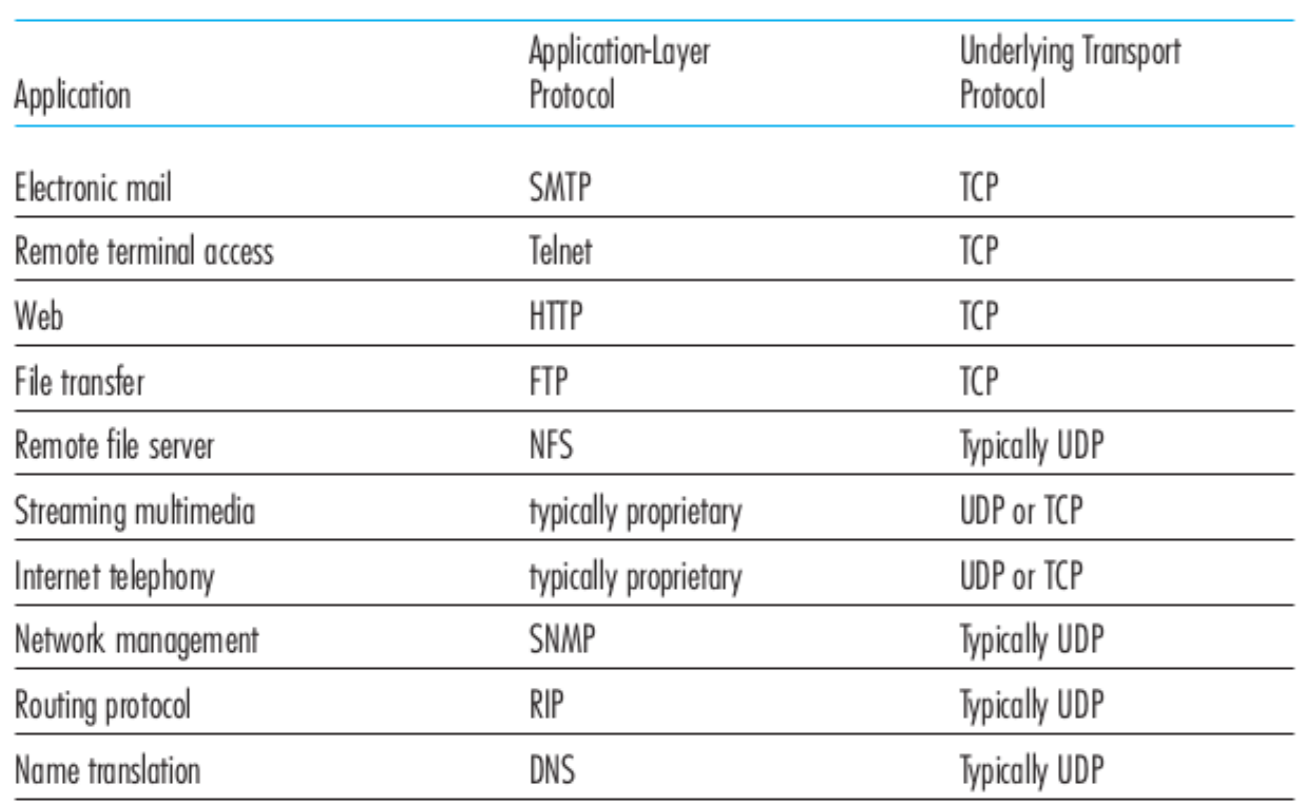
\includegraphics[width=12cm,height=6cm]{unit-18/figures/common-transport-protocols.png}
\end{table}

A UDP segment contains the source port number, destination port number, length of the UDP segment (including the header) in bytes, a checksum and the application data message.
UDP exists because it is simple.
There is no delay in establishing a connection, there is no connection state to maintain at the sender or receiver, UDP segments have a small header size and there is no congestion control mechanism (transfer rate is not limited).

\subsubsection{UDP Checksum}

A checksum exists to detect errors such as flipped bits in a transmitted segment.
The sender treats segment contents, including header fields, as a sequence of \SI{16}{\bit} integers.
It calculates a checksum as the one's complement of the sum of the segment contents.
The checksum is placed in the checksum field of the UDP segment.

The receiver computes the checksum of the received segment.
If the computed checksum is equal to the checksum field value, no error has been detected.
If the checksums are not equal, an error has been detected.
Even though the checksums may be equal, it does not necessarily mean that there is no error.

Given two \SI{16}{\bit} integers \(11110011001100110_2\) and \(1101010101010101_2\), their sum is the \SI{17}{\bit} integer \(11011101110111011_2\).
The overflow bit is removed from the sum and added to it as the least significant bit.
The sum of \(1_2\) and \(1011101110111011_2\) is \(1011101110111100_2\).
The one's complement (inverse) of this sum is \(0100010001000011_2\).
This is the checksum for the two integers.

\subsection{Principles of Reliable Data Transfer}

Although the service provided by a reliable transfer protocol may be that of transfer through a reliable channel, it may actually be implemented through an unreliable network layer channel.

\subsubsection[RDT over a Perfectly Reliable Channel (RDT1.0)]{Reliable Data Transfer over a Perfectly Reliable Channel (RDT1.0)}

If the underlying channel is perfectly reliable, i.e.\ there are no bit errors or loss of packets, reliable data transfer (RDT) can be accomplished by the sender transferring the data into packets to send through the unreliable channel.
At the receiver, the packets are extracted into a message that is delivered to the application layer.

\subsubsection[RDT over a Channel With Bit Errors (RDT2.0)]{Reliable Data Transfer over a Channel With Bit Errors (RDT2.0)}

If an underlying channel may flip bits in a packet, a checksum can be used to check bits.
Acknowledgements (ACKs) are sent from the receiver to the sender to indicate that the packet was received correctly.
Negative acknowledgements (NAKs) indicate that the received packet contained errors.
The sender retransmits the packet if it receives a NAK\@.

\subsubsection[RDT With Corrupted Acknowledgements (RDT2.1)]{Reliable Data Transfer With Corrupted Acknowledgements (RDT2.1)}

The flaw with RDT2.0 is that an ACK or NAK may itself be corrupted.
If the sender simply retransmits the packet when it receives a corrupted ACK/NAK, duplicate packets may be delivered.
Duplicates can be handled by adding a sequence number to each packet before it is sent.
The receiver discards a duplicate packet (one with a sequence number that has already been received).

This is a stop-and-wait implementation.
The sender sends a packet then waits for a response.
Thus, only two sequence numbers are required.
This implementation requires the sender to check whether acknowledgements are corrupted, and the receiver to check whether a received packet is a duplicate.
Both the sender and receiver must manage twice as many states as they must remember whether a packet should have a sequence number of \num{0} or \num{1}.

\subsubsection[RDT Without Negative Acknowledgements (RDT2.2)]{Reliable Data Transfer Without Negative Acknowledgements (RDT2.2)}

This achieves the same functionality as RDT2.1 using only ACKs.
The receiver responds with an ACK containing the sequence number of the last correctly received packet.
If the sender receives a duplicate ACK, it retransmits the current packet.

\subsubsection[RDT Over a Channel with Errors and Losses (RDT3.0)]{Reliable Data Transfer Over a Channel with Errors and Losses (RDT3.0)}

Assuming the underlying channel can also lose data packets, the use of checksums, sequence numbers, acknowledgements and retransmissions is not sufficient.
The sender must wait a reasonable amount of time for an ACK\@.
If no ACK is received in this time, the current packet is retransmitted.
If the ACK was delayed or lost, the retransmitted packet will be a duplicate.
This is already handled by sequence numbers.
This implementation requires the added complexity of a countdown timer.

Although RDT3.0 works correctly, it has poor performance.
For a \SI{1}{\giga\bit\per\second} link with a \SI{15}{\milli\second} propagation delay, an \SI{8000}{\bit} packet will have a transmission delay of \(d_{\text{trans}} = \frac{L}{R} = \frac{8000}{10^9} = 8 \times 10^{-6}\)~\si{\second}, and a sender utilisation of \(U_{\text{sender}} = \frac{\frac{L}{R}}{\text{RTT} + \frac{L}{R}} = \frac{8 \times 10^{-6}}{2 \times 15 \times 10^{-3} + 8 \times 10^{-6}} = 0.00027\).

This protocol limits the use of physical resources.
A solution is to use pipelined protocols.
A sender allows multiple ``in-flight'' yet to be acknowledged packets.
This requires the range of sequence numbers used to be increased.
The sender and receiver must have a buffer.

\subsection{Transmission Control Protocol (TCP)}

TCP provides point-to-point communication with one sender and one receiver.
It is a reliable protocol that sends an ordered byte stream.
TCP is pipelined with congestion and flow control to set the window size of available sequence numbers.
It allows full duplex data flow (bidirectional data flow in a single connection) and sets a maximum segment size (MSS).
It is connection-oriented --- handshaking initialises the sender and receiver states before data exchange.

\begin{figure}[htp]
  \centering
  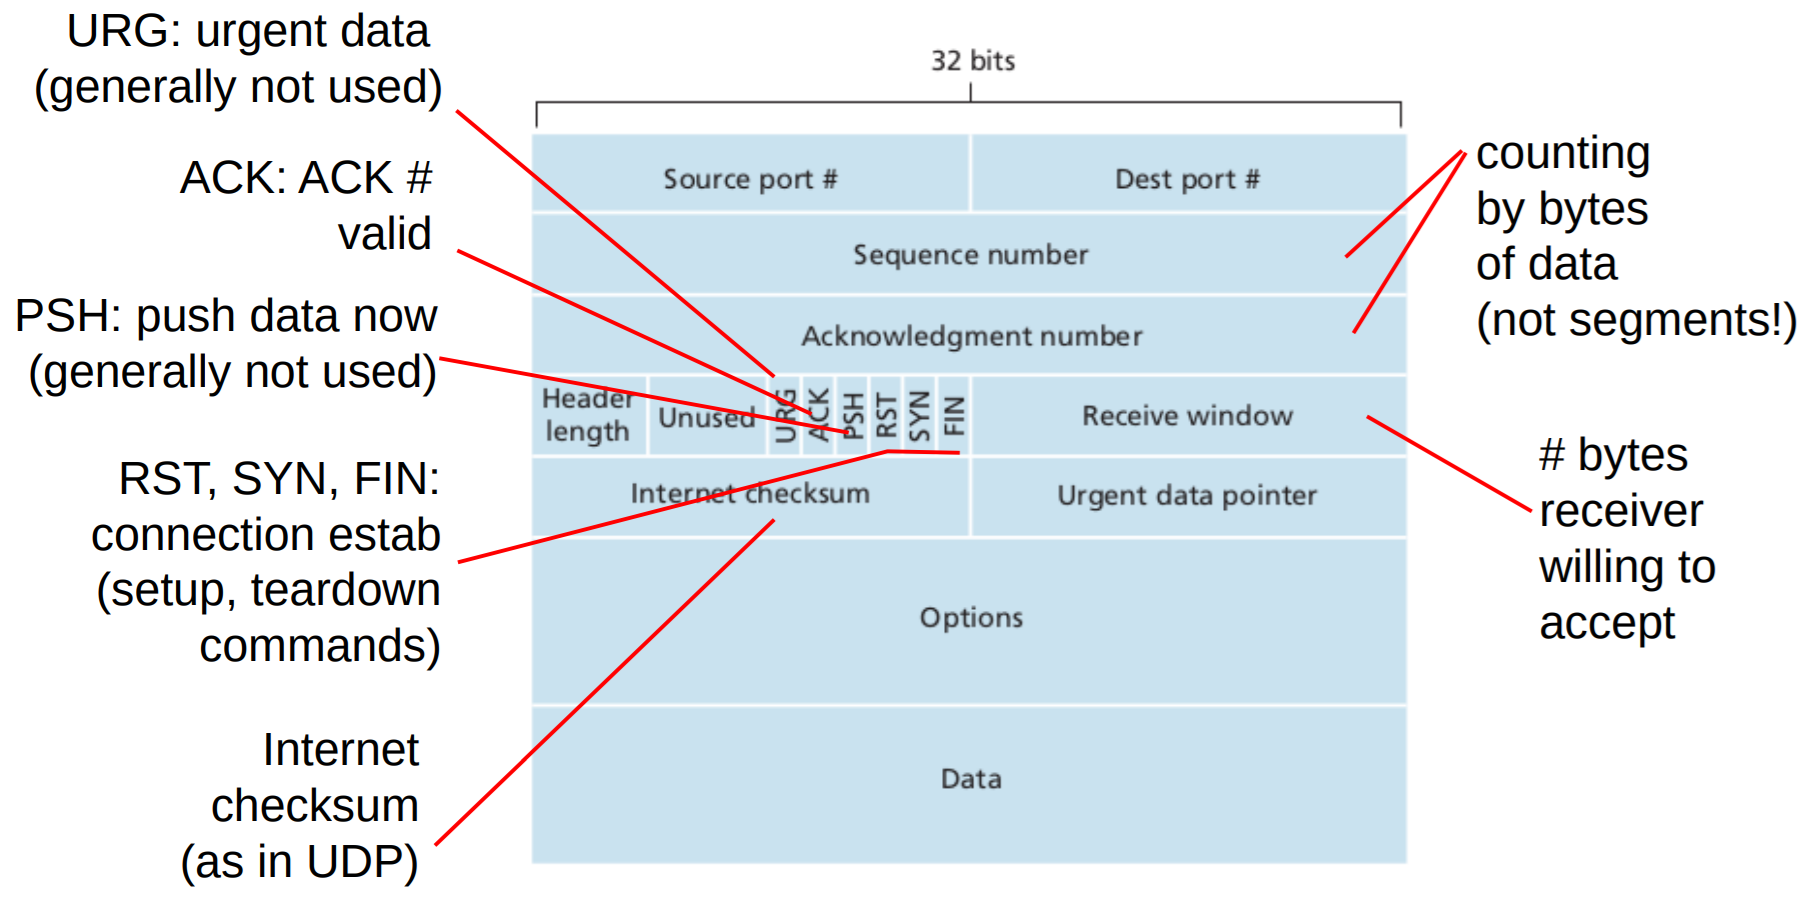
\includegraphics[width=15cm]{unit-18/figures/tcp-segment.png}
  \caption*{The structure of a TCP segment.}
\end{figure}

The sequence number of a TCP segment is the index of the first byte of data it contains.
The acknowledgement number of a TCP segment is the sequence number of the next segment expected from the other host.
This is known as `cumulative acknowledgement'.
The TCP specification does not state how out-of-order segments must be handled.
This is decided by the implementation.
Typically, out-of-order segments are kept.

\subsubsection{TCP Round-Trip Time and Timeout}

The TCP timeout interval should be longer than the RTT\@.
However, the RTT varies.
A timeout interval that is too short results in premature timeout and unnecessary retransmissions.
A timeout value that is too long will result in a slow reaction to segment loss.

RTT can be estimated using a sample RTT\@.
This is the measured time between segment transmission and acknowledgement receipt, ignoring retransmissions.
Since the sample RTT will vary, an exponential weighted moving average is used.

\begin{equation*}
  \text{estimated RTT} = \left( 1 - \alpha \right) \times \text{estimated RTT} + \alpha \times \text{sample RTT}
\end{equation*}

The influence of past samples decreases exponentially.
A typical value for the coefficient \(\alpha\) is \num{0.125}.

The timeout interval can be calculated as the sum of the estimated RTT and a safety margin.
A large variation in the estimated RTT should result in a larger safety margin.
Deviation of the sample RTT from the estimated RTT can be approximated.

\begin{equation*}
  \text{deviation} \approx (1 - \beta) \times \text{deviation} + \beta \times \left| \text{sample RTT} - \text{estimated RTT} \right|
\end{equation*}

A typical value for the coefficient \(\beta\) is \num{0.25}.

\begin{equation*}
  \text{timeout} = \text{estimated RTT} + 4 \times \text{deviation}
\end{equation*}

\subsubsection{TCP Retransmission Scenarios}

TCP creates a reliable data transfer service over the unreliable best-effort service of IP using pipelined segments, cumulative ACKs and a single retransmission timer.
Retransmissions are triggered by timeout events and duplicate ACKs.

\begin{enumerate}
  \item Create segment with sequence number --- sequence number is byte stream number of first data byte in segment
  \item Start timer if not already running --- timer corresponds to oldest unacknowledged segment
  \item On timeout, retransmit the segment and restart the timer
  \item On acknowledgement, update which segments are known to be acknowledged and start timer if there remain unacknowledged segments
\end{enumerate}

\begin{figure}[htp]
  \centering
  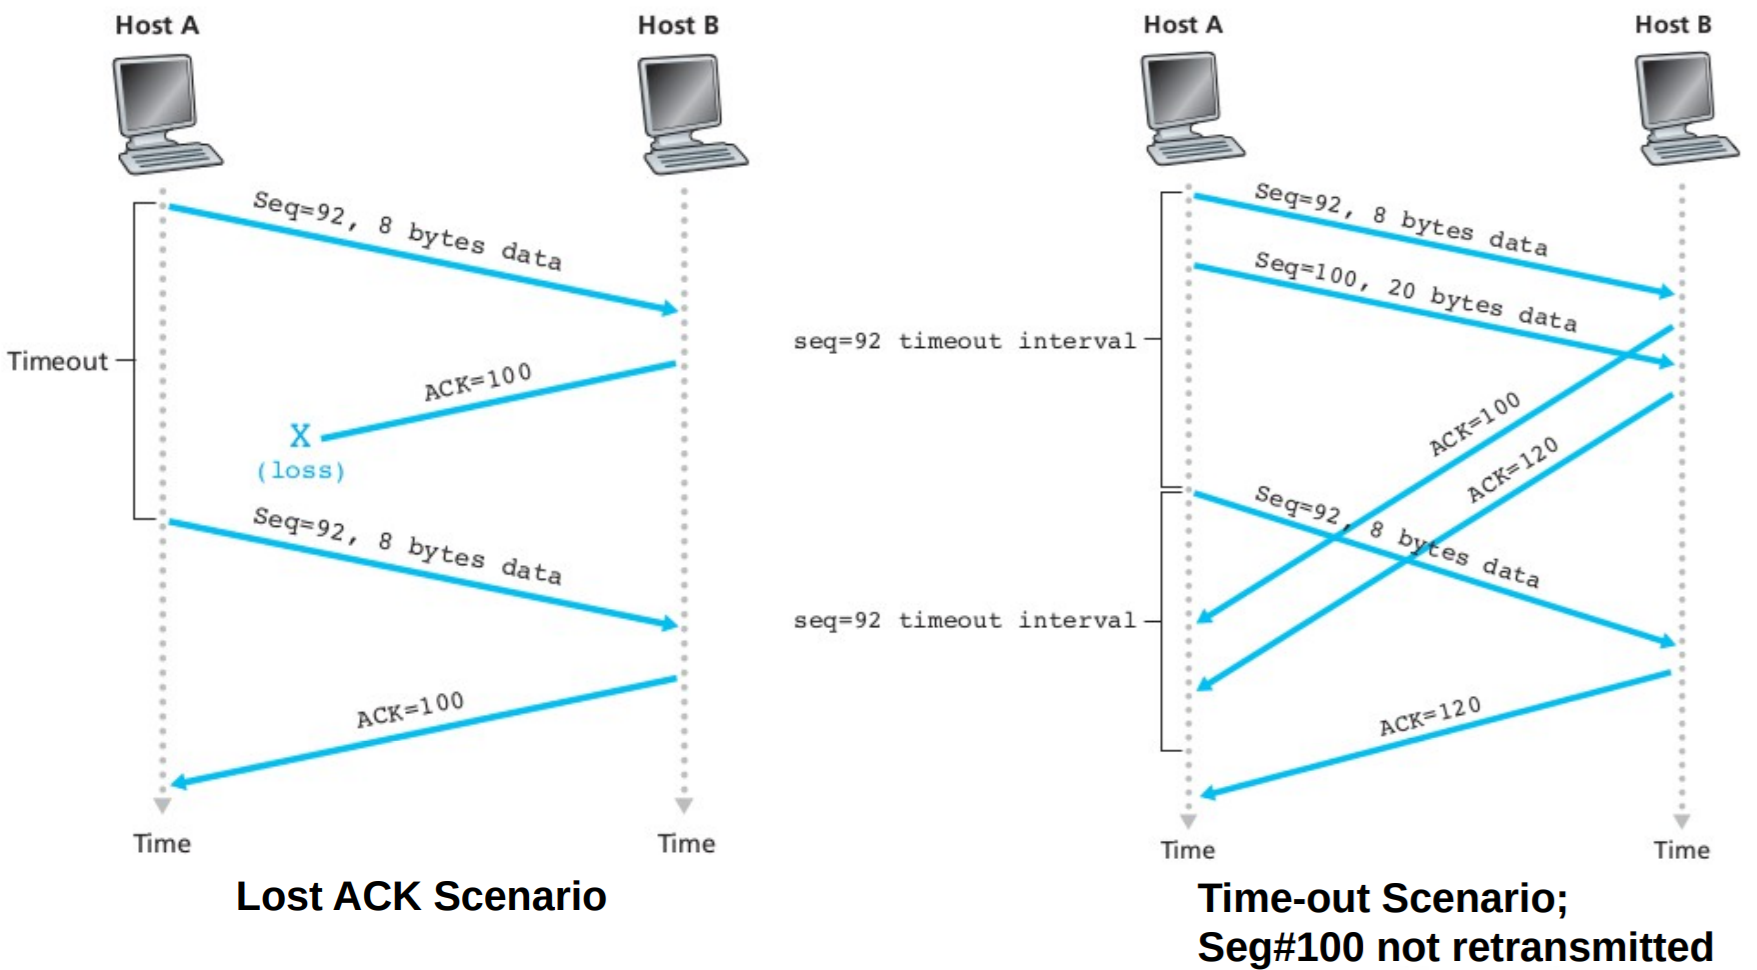
\includegraphics[width=15cm]{unit-18/figures/retransmission-scenarios-1.png}
  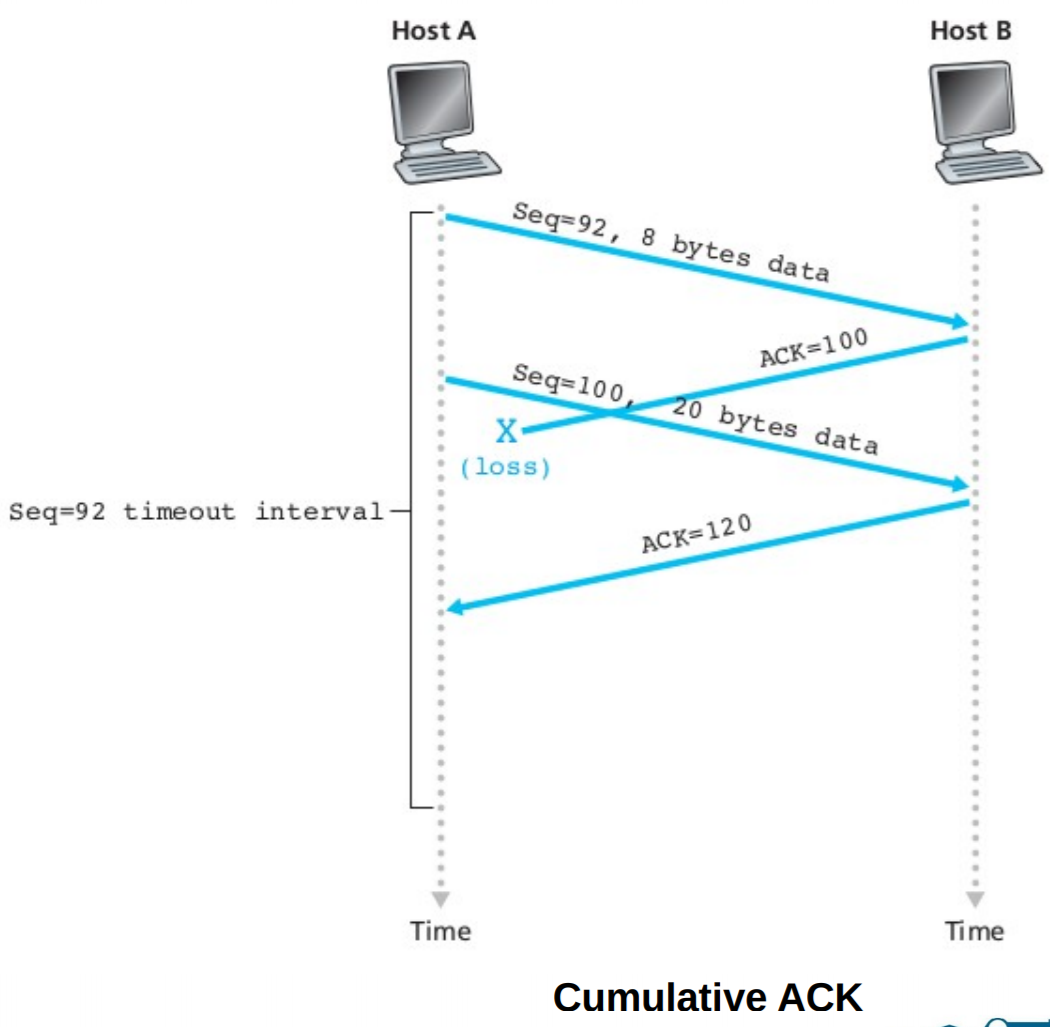
\includegraphics[width=10cm]{unit-18/figures/retransmission-scenarios-2.png}
  \caption*{TCP retransmission scenarios.}
\end{figure}

\begin{table}[htp]
  \centering
  \caption*{TCP acknowledgement generation.}
  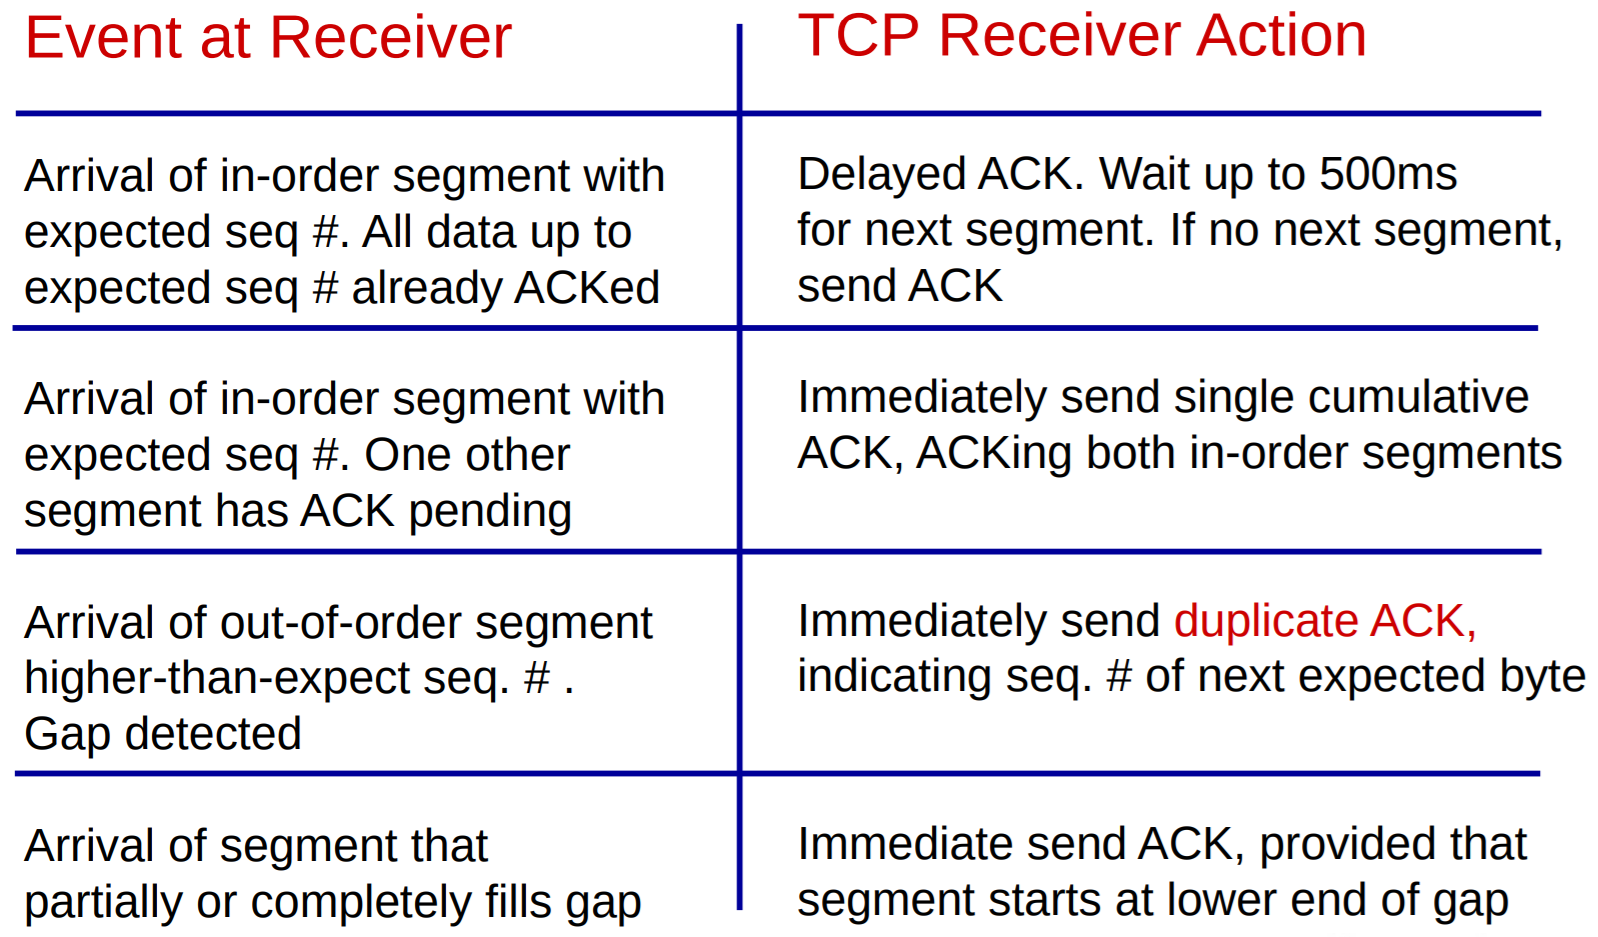
\includegraphics[width=10cm]{unit-18/figures/acknowledgement-generation.png}
\end{table}

\subsubsection{TCP Fast Retransmit}

Since the timeout period is relatively long, there may be a long delay before resending a lost packet.
Lost packets can be detected via duplicate ACKs.
If a segment is lost, there will likely be many duplicate ACKs.
If a sender receives three ACKs for the same data (``triple duplicate ACKs''), the unacknowledged segment with the smallest sequence number is resent.
Since the next few responses will likely indicate that the unacknowledged segment was lost, there is no need to wait for the timeout.

\subsubsection{TCP Flow Control}

The receiver controls the sender so that the sender does not overflow the buffer of the receiver by transmitting too much data too quickly.
The receiver advertises its free buffer space by including a receive window size in the TCP header of receiver-to-sender segments.
The receive buffer size is set via socket options.
Many operating systems automatically adjust the receive buffer.

The receiver sets the receive window size to the difference between receive buffer size and the difference between the number of bytes received and the number of bytes read.
The sender ensures that the difference between the last byte sent and the last byte acknowledged is less than or equal to the receive window size.
This ensures that the sender only sends an amount of data that can be handled by the receiver.

\begin{equation*}
  \text{receive window} = \text{receive buffer} - \left( \text{last byte received} - \text{last byte read} \right)
\end{equation*}

\begin{equation*}
  \text{last byte sent} - \text{last byte acknowledged} \le \text{receive window}
\end{equation*}

\subsubsection{TCP Connection Management}

Before exchanging data, the sender and receiver exchange a `handshake' through which they agree to establish a connection and agree on connection parameters.

\begin{figure}[htp]
  \centering
  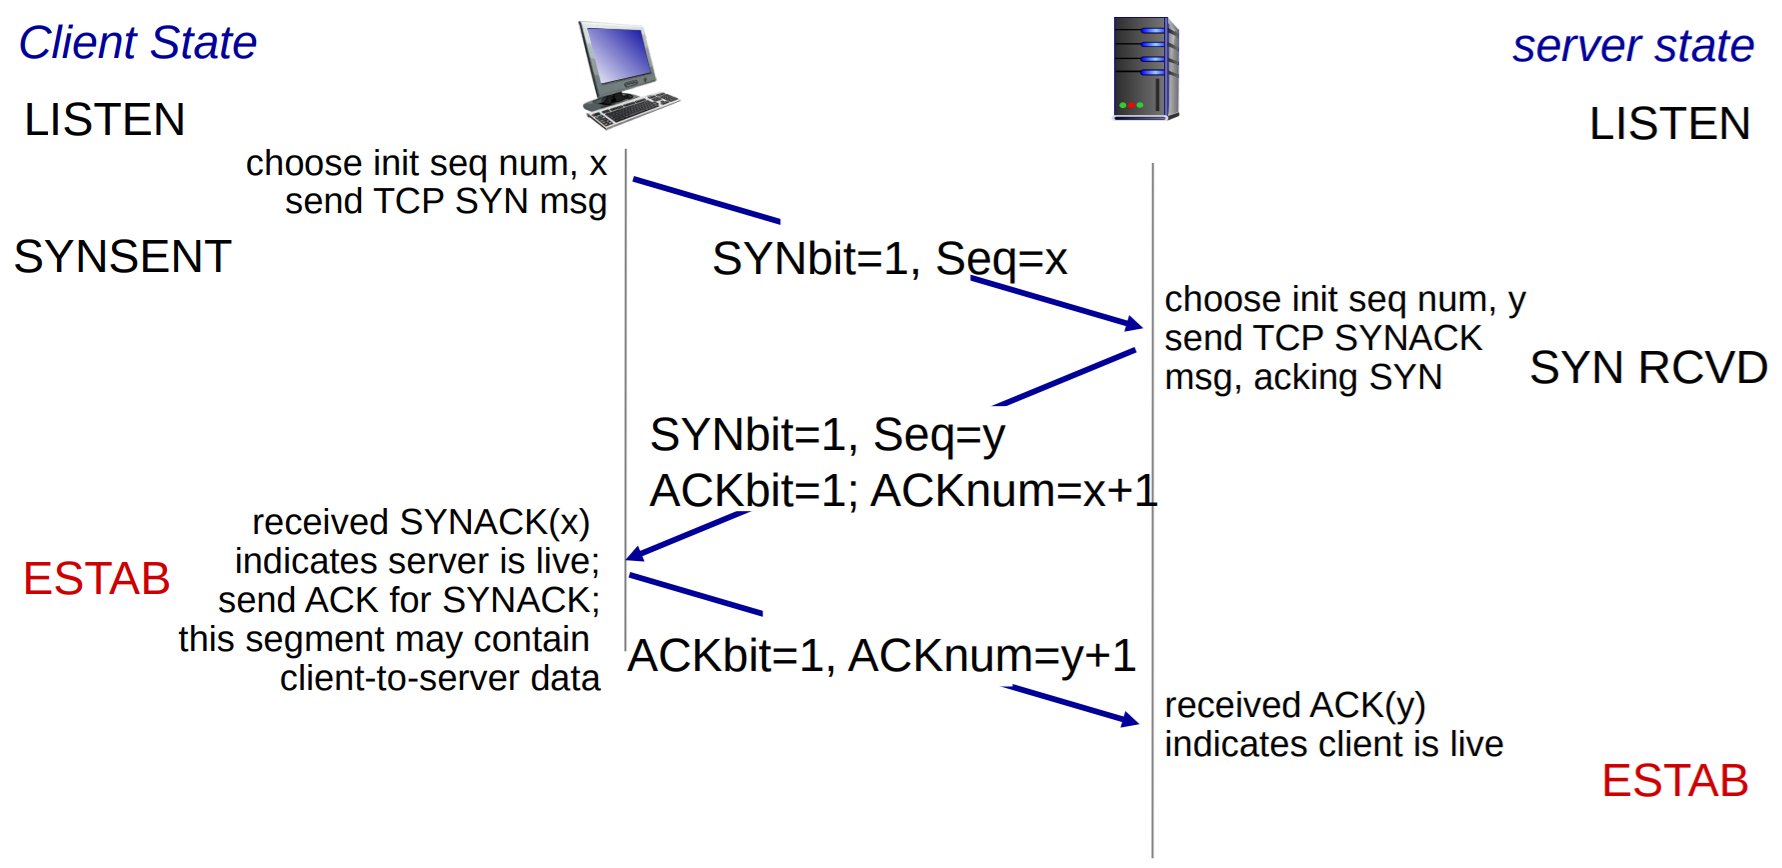
\includegraphics[width=12cm]{unit-18/figures/three-way-handshake.png}
  \caption*{The TCP three-way handshake.}
\end{figure}

When a TCP connection is closed, the client and server both close their side of the connection by sending a TCP segment with a FIN bit of \num{1}.
When a host receives a FIN message, it replies with an ACK\@.
When the host is ready to close the connection it sends another FIN message and receives an ACK\@.
The TCP connection is now closed.
Simultaneous FIN exchanges can be handled.

\begin{figure}[htp]
  \centering
  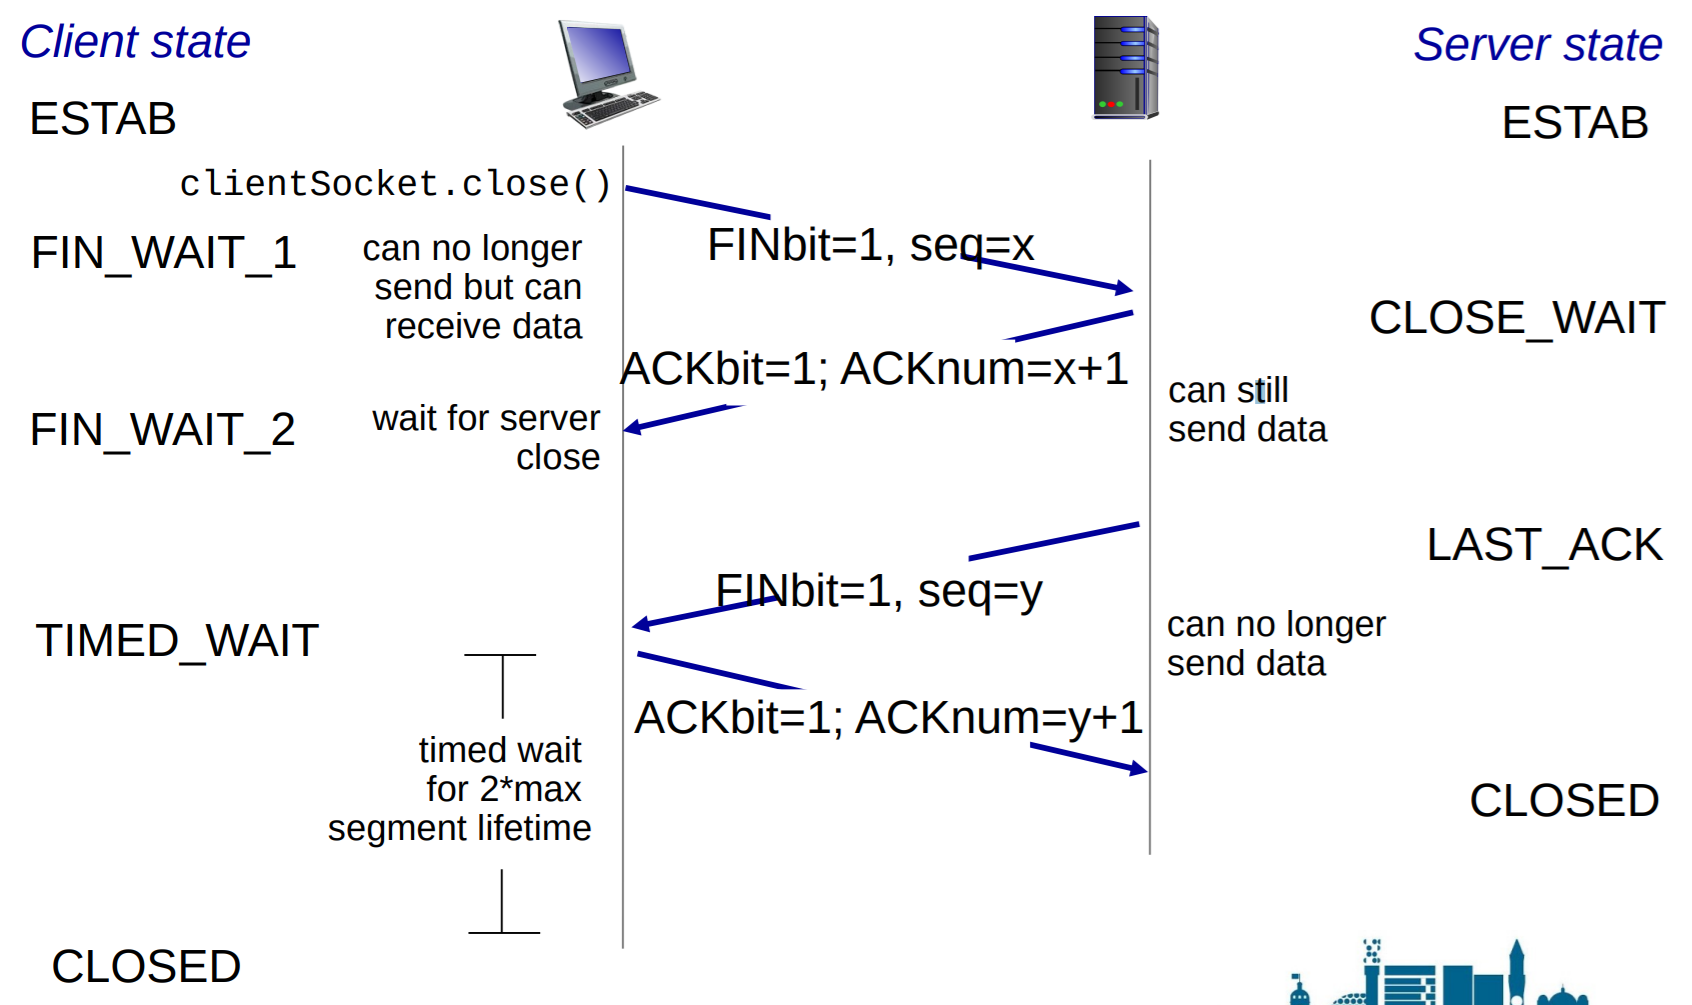
\includegraphics[width=12cm]{unit-18/figures/closing-connection.png}
  \caption*{Closing a TCP connection.}
\end{figure}
